\chapter{The SpiNNaker Architecture}
	
	\label{sec:background}
	
	SpiNNaker is a massively parallel computer architecture designed to simulate
	biologically realistic neural models \cite{furber07}. In this chapter we will
	explore this unconventional architecture in detail, starting with its purpose
	before focusing on its most unconventional feature: its network.
	
	% * Purpose
	%   * Spiking neural simulations
	%     * Neural modelling: PyNN, Nengo...
	%     * Parallelisation + communication
	
	\section{Neural simulation}
		
		Human brains contain billions of neurons connected together by trillions of
		synapses. The neurons communicate by transmitting and receiving `spikes'
		through their synapses. Each spike is `valueless' in that a spike's only
		significant features are when it arrives and where it has come from.
		
		\begin{figure}
			\center
			\buildfig{figures/lif-neuron.tex}
			
			\caption{A Leaky Integrate-and-Fire (LIF) neuron.}
			\label{fig:lif-neuron}
		\end{figure}
		
		Though some detailed models of the electrochemical processes occurring
		inside neurons are computationally intensive, simplified models such as the
		Leaky Integrate-and-Fire (LIF) model can be implemented in just a handful
		of CPU instructions\footnote{Or, in the case of
		figure~\ref{fig:lif-neuron}, seven lines of \LaTeX{} macros.}
		\cite{vainbrand11}. Figure~\ref{fig:lif-neuron} illustrates a simple LIF
		neuron in which incoming spikes cause charge to build up (integrated) which
		over time, leaks away. If an incoming spike causes the charge to rise above
		a certain threshold, the neuron `fires' producing a spike. Despite the
		simplicity of this model, large neural networks such as Spaun
		\cite{eliasmith12} -- built entirely from LIF neurons -- exhibit complex
		behaviours such as fine motor control and problem solving.
		
		The computational expense of large scale neural simulations does not arise
		from the cost of modelling neurons but instead from distributing spikes. In
		biology, neurons produce spikes at an average rate of \SI{10}{\hertz} and
		synapses connect each neuron's output to (order) \num{1000}~neurons
		\cite{navaridas09}. Consider an example neural model with $7\times10^7$
		neurons, approximately the number in a house mouse and
		$\nicefrac{1}{10}^\textrm{th}$ of the design target of SpiNNaker. This
		network might produce $7\times10^8$~spikes per second. Because each neuron
		connects to many others, this equates to $7\times10^{11}$ spikes being
		received per second. If each spike were transmitted as a UDP datagram
		containing a single \SI{32}{\bit} payload, the total network throughput
		required for this simulation would be \SI{179.2}{\tera\bit\per\second}. At
		the time of writing, this is more than double the bisection bandwidth (the
		theoretical worst-case throughput) of the world's most powerful super
		computer \cite{dongarra16}.
	
	\section{Network architecture}
		
		Architectures such as IBM's Blue Gene \cite{chiu11} and Cray's XK7
		\cite{ornl16} employ powerful compute nodes connected together using
		networks designed to transfer multi-kilobyte blocks of data between nodes.
		Since neural models have relatively light computational requirements and
		communications are based on small pieces of data (spikes), this type of
		architecture is poorly suited to the task.
		
		SpiNNaker's architectural target is to support realtime simulations of up
		to one billion neurons. Since neural models such as LIF are inexpensive to
		model and many neurons can be simulated independently in parallel,
		SpiNNaker employs many small, energy efficient ARM processors
		\cite{furber07}. To support the unusual communication requirements of
		neural simulations, a bespoke interconnection network is used which is the
		subject of this thesis.
		
	%   * SpiNNaker chip
	%     * Cores
	%     * SDRAM
	%     * NoC
	%     * Router
		
		\begin{figure}
			\center
			%
\includegraphics[width=19mm]{figures/spinnakerChip.jpg}
			\buildfig{figures/hex-chips.tex}
			
			\caption[SpiNNaker chips connected to their six neighbours.]%
			{SpiNNaker chips (actual size) connected to their six neighbours.}
			\label{fig:spinnakerChip}
		\end{figure}
		
		The fundamental building block of the SpiNNaker architecture is the
		SpiNNaker chip (figure \ref{fig:spinnakerChip}) \cite{furber13}. Each chip
		contains eighteen low power ARM 968 processor cores each capable of
		simulating between \num{200} and \num{2000} LIF neurons in real time
		\cite{mundy15}.  Each core has a total of \SI{96}{\kilo\byte} of private
		Tightly-Coupled Memory (TCM) and shares access to \SI{128}{\mega\byte} of
		on-chip SDRAM with other cores on the same chip. Finally, each chip
		contains a programmable router which routes network packets to and from the
		local cores and six neighbouring SpiNNaker chips. SpiNNaker machines are
		constructed by combining many SpiNNaker chips.
		
		\begin{figure}
			\center
			\buildfig{figures/spinnaker-packet.tex}
			
			\caption{SpiNNaker's \SI{40}{\bit} and \SI{72}{\bit} multicast packet
			format.}
			\label{fig:spinnaker-packet}
		\end{figure}
		
		Processor cores can communicate by sending and receiving network packets
		forwarded by routers through the network. Since SpiNNaker's network is
		designed to efficiently transmit neural spike events, individual network
		packets are small, either \SI{40}{\bit} or \SI{72}{\bit} compared with tens
		or hundreds of bytes in typical network architectures.
		
		In a real-time simulation, the time at which a spike is produced is
		implicitly indicated by the time it is received -- since at biological
		timescales a computer network delivers packets `instantaneously'.
		Consequently, the only information which must be explicitly encoded is the
		identity of the neuron which produced the spike. In SpiNNaker, a spike may
		be encoded by using a single \SI{40}{\bit} `multicast packet' whose format
		is illustrated in figure~\ref{fig:spinnaker-packet}.  The \SI{8}{\bit}
		header is used by SpiNNaker's routers to determine the type of packet and
		the \SI{32}{\bit} `routing key' is used to uniquely identify the neuron
		which produced the packet. The routing key is also used by SpiNNaker's
		routers to determine how the packet should be directed through the network.
		
		The optional \SI{32}{\bit} payload is not used by conventional spiking
		neural simulations \cite{galluppi10} but has been exploited to enable more
		efficient simulation of a particular class of neural models \cite{mundy15}.
	
	\section{The SpiNNaker router}
		
		The SpiNNaker router employs an unconventional design which, despite its
		compact size and small energy requirements, implements a flexible multicast
		routing scheme. Unlike conventional routers which often employ hard-coded
		routing rules \cite{dally04}, the SpiNNaker router uses a programmable
		`routing table' to determine how packets should be forwarded.
		
		In addition, to avoid deadlocks, SpiNNaker's router employs a simple
		timeout-based mechanism which exploits the ability of neural networks to
		tolerate occasional missing packets. As we will see in chapter
		\ref{sec:routing}, this mechanism greatly simplifies the task
		of routing in SpiNNaker's network.
		
		In this section we'll see how both of these distinctive features of
		SpiNNaker's router are used.
		
		\subsection{Routing tables}
		
			When a multicast packet arrives at a SpiNNaker router (either from a
			local core or a neighbouring chip), the router looks up the routing key
			in its routing table. This table consists of \num{1024} programmable
			table entries, each specifying a routing key bit pattern to match and a
			set of routes.  When a multicast packet's key is matched by a routing
			entry the packet is forwarded along every route specified by that entry,
			potentially duplicating the packet. This `multicast' technique allows
			packets to be transmitted once but received in a number of places while
			making efficient use of the network \cite{navaridas12}.
			
			Though routing table entries are in finite supply (\num{1024} entries per
			router), it is still possible for many thousands of traffic flows to be
			routed through a single router. The bit pattern in each routing entry
			matches against the 32~bits of a routing key as either `\texttt{1}',
			`\texttt{0}' or `\texttt{X}' (don't care).  This means that a single
			routing entry may, for example, be used to match all routing keys with a
			certain prefix. If a routing key is not matched by any entry in the
			routing table then the packet is `default routed' in a straight line. For
			example if a packet with an unmatched key is received from the chip to
			the left, the packet will be default routed to the chip on the right. By
			assigning routing keys such that neurons whose spikes are sent to similar
			destinations share a similar prefix, the number of routing entries
			required by a simulation is greatly reduced \cite{davies12}.
			
			\begin{figure}
				\center
				\buildfig{figures/routing-example.tex}
				
				\caption[Multicast routing example.]%
				{Multicast routing example with \SI{4}{\bit} routing keys. Each
				box represents a SpiNNaker chip whose router has been programmed with
				the routing entries shown. Grey lines mark connections between chips.}
				\label{fig:routing-example}
			\end{figure}
			
			Consider the simplified example in figure~\ref{fig:routing-example} in
			which a number of (\SI{4}{\bit}) routing table entries have been
			configured in the routers of a small SpiNNaker network. If a packet with
			the routing key \texttt{1011} is transmitted by a core in the chip
			labelled $(0, 0, 0)$, this will match the first routing table entry on
			that chip and will be routed to chip $(1, 0, 0)$. On chip $(1, 0, 0)$,
			the packet once again matches the first routing entry and is routed to
			chip $(1, 0, -1)$. On $(1, 0, -1)$, no match is made so the packet is
			default routed to $(1, 0, -2)$. On this chip, the packet matches a
			routing entry which routes the packet to core~7. In this example, default
			routing allows only three routing table entries to direct a packet
			through four chips.
			
			As a second example, if a packet with the routing key \texttt{0010} is
			transmitted by a core on chip $(0, 0, 0)$, this key will be matched by
			the second routing entry since \texttt{X}s in the table entry will match
			both \texttt{1}s and \texttt{0}s in the corresponding bits of the routing
			key. When the packet arrives at chip $(0, 0, -1)$ the matching routing
			entry forwards the packet to both $(0, 1, -1)$ and $(1, 0, -1)$
			simultaneously. The copy of the packet arriving at $(0, 1, -1)$ is routed
			to core~5 on that chip.  Meanwhile, the copy forwarded to $(1, 0, -1)$ is
			duplicated again with one copy being routed to core~11 and another being
			routed to chip $(1, 0, -2)$. Here the packet is finally delivered to
			core~6. In this example, the ability of the router to multicast
			(duplicate) packets as they pass through the network meant that sending
			one copy of the packet was sufficient to reach three destination cores.
			In addition, by using \texttt{X}s in the routing table entry, the same
			routing entries are sufficient to route packets with the keys
			\texttt{0000}, \texttt{0001}, \texttt{0010} and \texttt{0011}.
			
			In spite of these mechanisms, it is still possible for an application to
			run out of routing table entries. As we will see in
			chapter~\ref{sec:placement} by arranging applications appropriately
			within SpiNNaker's network, routing table usage can be reduced. In
			addition, other behaviours of SpiNNaker's router may be exploited to
			compress an applications routing tables further, however the techniques
			employed are beyond the scope of this thesis \cite{mundy16}.
		
		\subsection{Timeouts}
			
			\begin{figure}
				\center
				\buildfig{figures/router-architecture.tex}
				
				\caption{SpiNNaker router architecture}
				\label{fig:router-architecture}
			\end{figure}
			
			SpiNNaker's router is built on a pipeline architecture. As shown in
			figure~\ref{fig:router-architecture}, the router is fed packets by an
			arbiter which serialises packets arriving from other chips and local
			cores. Every (\SI{100}{\mega\hertz}) clock cycle, the router pipeline
			accepts one packet from the arbiter and routes a packet to one or several
			output links. If any of the required output ports are busy then the
			packet is not forwarded to any output link and the pipeline stalls. Once
			a packet has been blocked for a programmable timeout, it is dropped
			(discarded) and routing continues as usual for next packet in the
			pipeline. Links become blocked while transmitting packets or waiting for
			the remote receiver to become ready. For example, a receiving processor
			core may be busy performing some computation or a receiving router may be
			blocked waiting for some of its outputs to become ready.
			
			The timeout-based packet dropping mechanism is designed to defuse
			deadlocks in the network. For example, if two routers are trying to send
			each other a packet at the same time they may become deadlocked, each
			waiting for the other router to accept a packet before processing any
			other packets. SpiNNaker's timeout mechanism breaks deadlocks by dropping
			the packets which have been blocked for some time and therefore may be in
			a deadlock. Once a packet has been dropped it is left to the software to
			either tolerate the missing packet or trigger a retransmission. In neural
			simulations, as in biology, the loss of a single spike is unlikely to
			have a significant impact on the behaviour of a neural model and
			therefore these simulations are inherently tolerant of occasional dropped
			packets. During application loading and other system tasks, a higher
			level software driven protocol based on acknowledgements and
			retransmissions is used to ensure guaranteed delivery.
			
			% TODO: MENTION TIMEOUT VALUE USED?
			% Router timeouts must be configured to be long enough that delays in
			% packet transmission, for example due to the time taken for packets to
			% traverse a link, do not trigger packet dropping. Conversely, the timeout
			% should be as short as possible to reduce the time the router is
			% blocked and maximise network throughput.
	
	\section{The hexagonal torus topology}
		
		Each SpiNNaker chip is a node in a `hexagonal torus topology' as
		illustrated in figure~\ref{fig:hexagonalTorusTopology}. Network packets
		sent by SpiNNaker's processor cores may `hop' through several nodes in the
		network to reach their intended destination. In each hop, a packet may
		advance one node along one of the three axes of the topology. For example,
		a packet sent by the node labelled $\alpha$ (in the bottom-left corner) to
		the node labelled $\beta$, might take the following sequence of hops:
		X$^+$, X$^+$, Z$^-$. Packets sent from $\alpha$ to $\gamma$ might take the
		route: X$^-$, X$^-$, Y$^+$, Y$^+$. The first hop of this route `wraps
		around' from the bottom-left node to the bottom-right node in a single hop.
		
		\begin{figure}
			\center
			\buildfig{figures/hexagonalTorusTopology.tex}
			
			\caption[A hexagonal torus topology.]%
			{A hexagonal torus topology. Each hexagon represents a node (i.e.
			a SpiNNaker chip). Touching nodes are directly connected. Nodes on edges
			$a$, $b$ and $c$ are also directly connected to the corresponding nodes
			on edges $a'$, $b'$ and $c'$, respectively. The three axes of the
			hexagonal torus topology, `X', `Y' and `Z' are also shown.}
			\label{fig:hexagonalTorusTopology}
		\end{figure}
		
		\begin{figure}
			\center
			\begin{subfigure}{0.39\linewidth}
				\center
				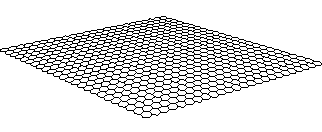
\includegraphics[width=\linewidth]{figures/torus-3d-flat.pdf}
				\caption{}
				\label{fig:torus-3d-flat}
			\end{subfigure}
			~~
			\begin{subfigure}{0.26\linewidth}
				\center
				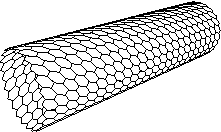
\includegraphics[width=\linewidth]{figures/torus-3d-tube.pdf}
				\caption{}
				\label{fig:torus-3d-tube}
			\end{subfigure}
			~~
			\begin{subfigure}{0.23\linewidth}
				\center
				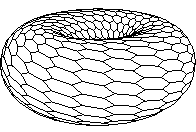
\includegraphics[width=\linewidth]{figures/torus-3d-torus.pdf}
				\caption{}
				\label{fig:torus-3d-torus}
			\end{subfigure}
			
			\caption{Visualisation of a hexagonal torus topology as a torus.}
			\label{fig:torus-3d}
		\end{figure}
		
		The wrap around connections in the topology are what give it the `torus'
		part of its name. Figure~\ref{fig:torus-3d-flat} shows a hexagonal torus
		topology drawn flat as in the previous figure. If the topology is rolled up
		into a tube such that the top and bottom nodes become directly adjacent, a
		tube is formed as in figure~\ref{fig:torus-3d-tube}. This tube can then be
		bent to bring together the nodes at the ends of the tube to form a torus as
		shown in figure~\ref{fig:torus-3d-torus}.
		
		A hexagonal torus topology is typically defined in terms of its width and
		height along the X and Y axes respectively. For example,
		figure~\ref{fig:hexagonalTorusTopology} shows a $10\times10$ hexagonal
		torus.  The nodes in a hexagonal torus topology are addressed using
		hexagonal coordinates of the form $(x, y, z)$ \cite{patel15}. The bottom
		left node (labelled $\alpha$ in the figure) has the coordinate $(0, 0, 0)$
		and other nodes are assigned coordinates according to the number of hops
		along each dimension from $(0, 0, 0)$, for example node $\beta$ has the
		coordinate $(2, 0, -1)$.
		
		Counter intuitively, individual nodes in hexagonal torus topologies may be
		described by many different coordinates, for example $(3, 1, 0)$ and $(1,
		-1, -2)$ are also valid coordinates for node $\beta$. These dual
		coordinates emerge from the fact that adding $(1, 1, 1)$ to a coordinate
		produces an equivalent, but different, coordinate. This phenomenon is
		explained in detail in appendix~\ref{app:minimal-hex-coordinates} and
		related phenomena will be discussed in chapter~\ref{sec:shortestPaths}.
		
		\begin{figure}
			\center
			\begin{subfigure}[b]{0.32\linewidth}
				\center
				\buildfig{figures/torus-compare-hexagonal.tex}
				
				\caption{Hexagonal}
				\label{fig:torus-compare-hexagonal}
			\end{subfigure}
			\begin{subfigure}[b]{0.32\linewidth}
				\center
				\buildfig{figures/torus-compare-2d.tex}
				
				\caption{2D}
				\label{fig:torus-compare-2d}
			\end{subfigure}
			\begin{subfigure}[b]{0.32\linewidth}
				\center
				\buildfig{figures/torus-compare-3d.tex}
				
				\caption{3D}
				\label{fig:torus-compare-3d}
			\end{subfigure}
			
			\caption[Visual comparison of torus topologies.]%
			{Visual comparison of torus topologies. In all figures, `wrap
			around' connections between nodes at the ends of each axis are omitted
			for clarity.}
			\label{fig:torus-compare}
		\end{figure}
		
		Despite its unusual coordinate system, hexagonal torus topologies compare
		favourably with more conventional network topologies such as 2D and 3D
		toruses (sometimes known as 2-ary $N$-cubes and 3-ary $N$-cubes
		respectively) \cite{dally04} illustrated in figure~\ref{fig:torus-compare}.
		Compared with the 2D torus topology, a hexagonal torus has double the
		bisection bandwidth even though it only requires 50\% more node-to-node
		links \cite{navaridas09}.  Compared with a 3D torus topology, however, the
		hexagonal torus topology has half the bisection bandwidth even though each
		node has the same number of links. Once embedded into a real world data
		centre, however, three, and higher-dimensional (and higher) torus
		topologies become more expensive to construct in practice.  Since large
		machine rooms approximate a 2D space, longer cables are required to
		interconnect nodes which are adjacent in the higher dimensional space of
		the network but not in a 2D projection. As chapter~\ref{sec:building}
		demonstrates, hexagonal toruses may be assembled in a machine room -- in a
		similar way to a 2D topology -- using only short cables. Overall, the
		hexagonal torus topology achieves the scalability of a 2D torus while
		gaining some of the bisection bandwidth benefits of the 3D torus topology.
		
		Most torus topologies, including hexagonal 2D and 3D toruses, are related
		to an equivalent `mesh' topology. Mesh topologies maintain the same general
		connectivity structure as the corresponding torus topology with the
		exception of wrap-around links which are omitted. Omitting wrap-around
		links in practice saves a small number of links at the expense of halving
		the network's bisection bandwidth. As a consequence, mesh topologies are
		rarely used.
		
		\begin{figure}
			\center
			\begin{subfigure}[b]{0.45\linewidth}
				\center
				\buildfig{figures/hexagonal-torus.tex}
				\caption{Hexagonal torus}
				\label{fig:topo-compare-hexagonal-torus}
			\end{subfigure}
			\begin{subfigure}[b]{0.45\linewidth}
				\center
				\buildfig{figures/h-torus.tex}
				\caption{H-torus}
				\label{fig:topo-compare-h-torus}
			\end{subfigure}
			
			\caption[Hexagonal torus vs. H-torus topology.]%
			{Hexagonal torus vs. H-torus topology. Each numbered hexagon
			represents a node. The thick outline indicates the bounds of the
			topology after which the network repeats. In each topology, the path
			taken by advancing in the Y$^+$ direction from the node labelled `0' is
			shown.}
			\label{fig:topo-compare}
		\end{figure}
		
		\label{sec:hex-vs-h-torus}
		
		The hexagonal torus topology is not to be confused with the `H-torus'
		topology. This topology also uses a hexagonal tiling of nodes and even
		wraps this tiling into a torus-like topology \cite{zhao08}. However,
		H-torus topologies have very different characteristics to the hexagonal
		torus topology and are related to `twisted torus' topologies
		\cite{camara10}. For example, figure~\ref{fig:topo-compare} illustrates one
		major difference in the way paths wrap around the peripheries of both
		topologies.
	
	\section{Scaling-up SpiNNaker machines}
		
		\begin{figure}
			\center
			\begin{subfigure}[b]{0.45\linewidth}
				\center
				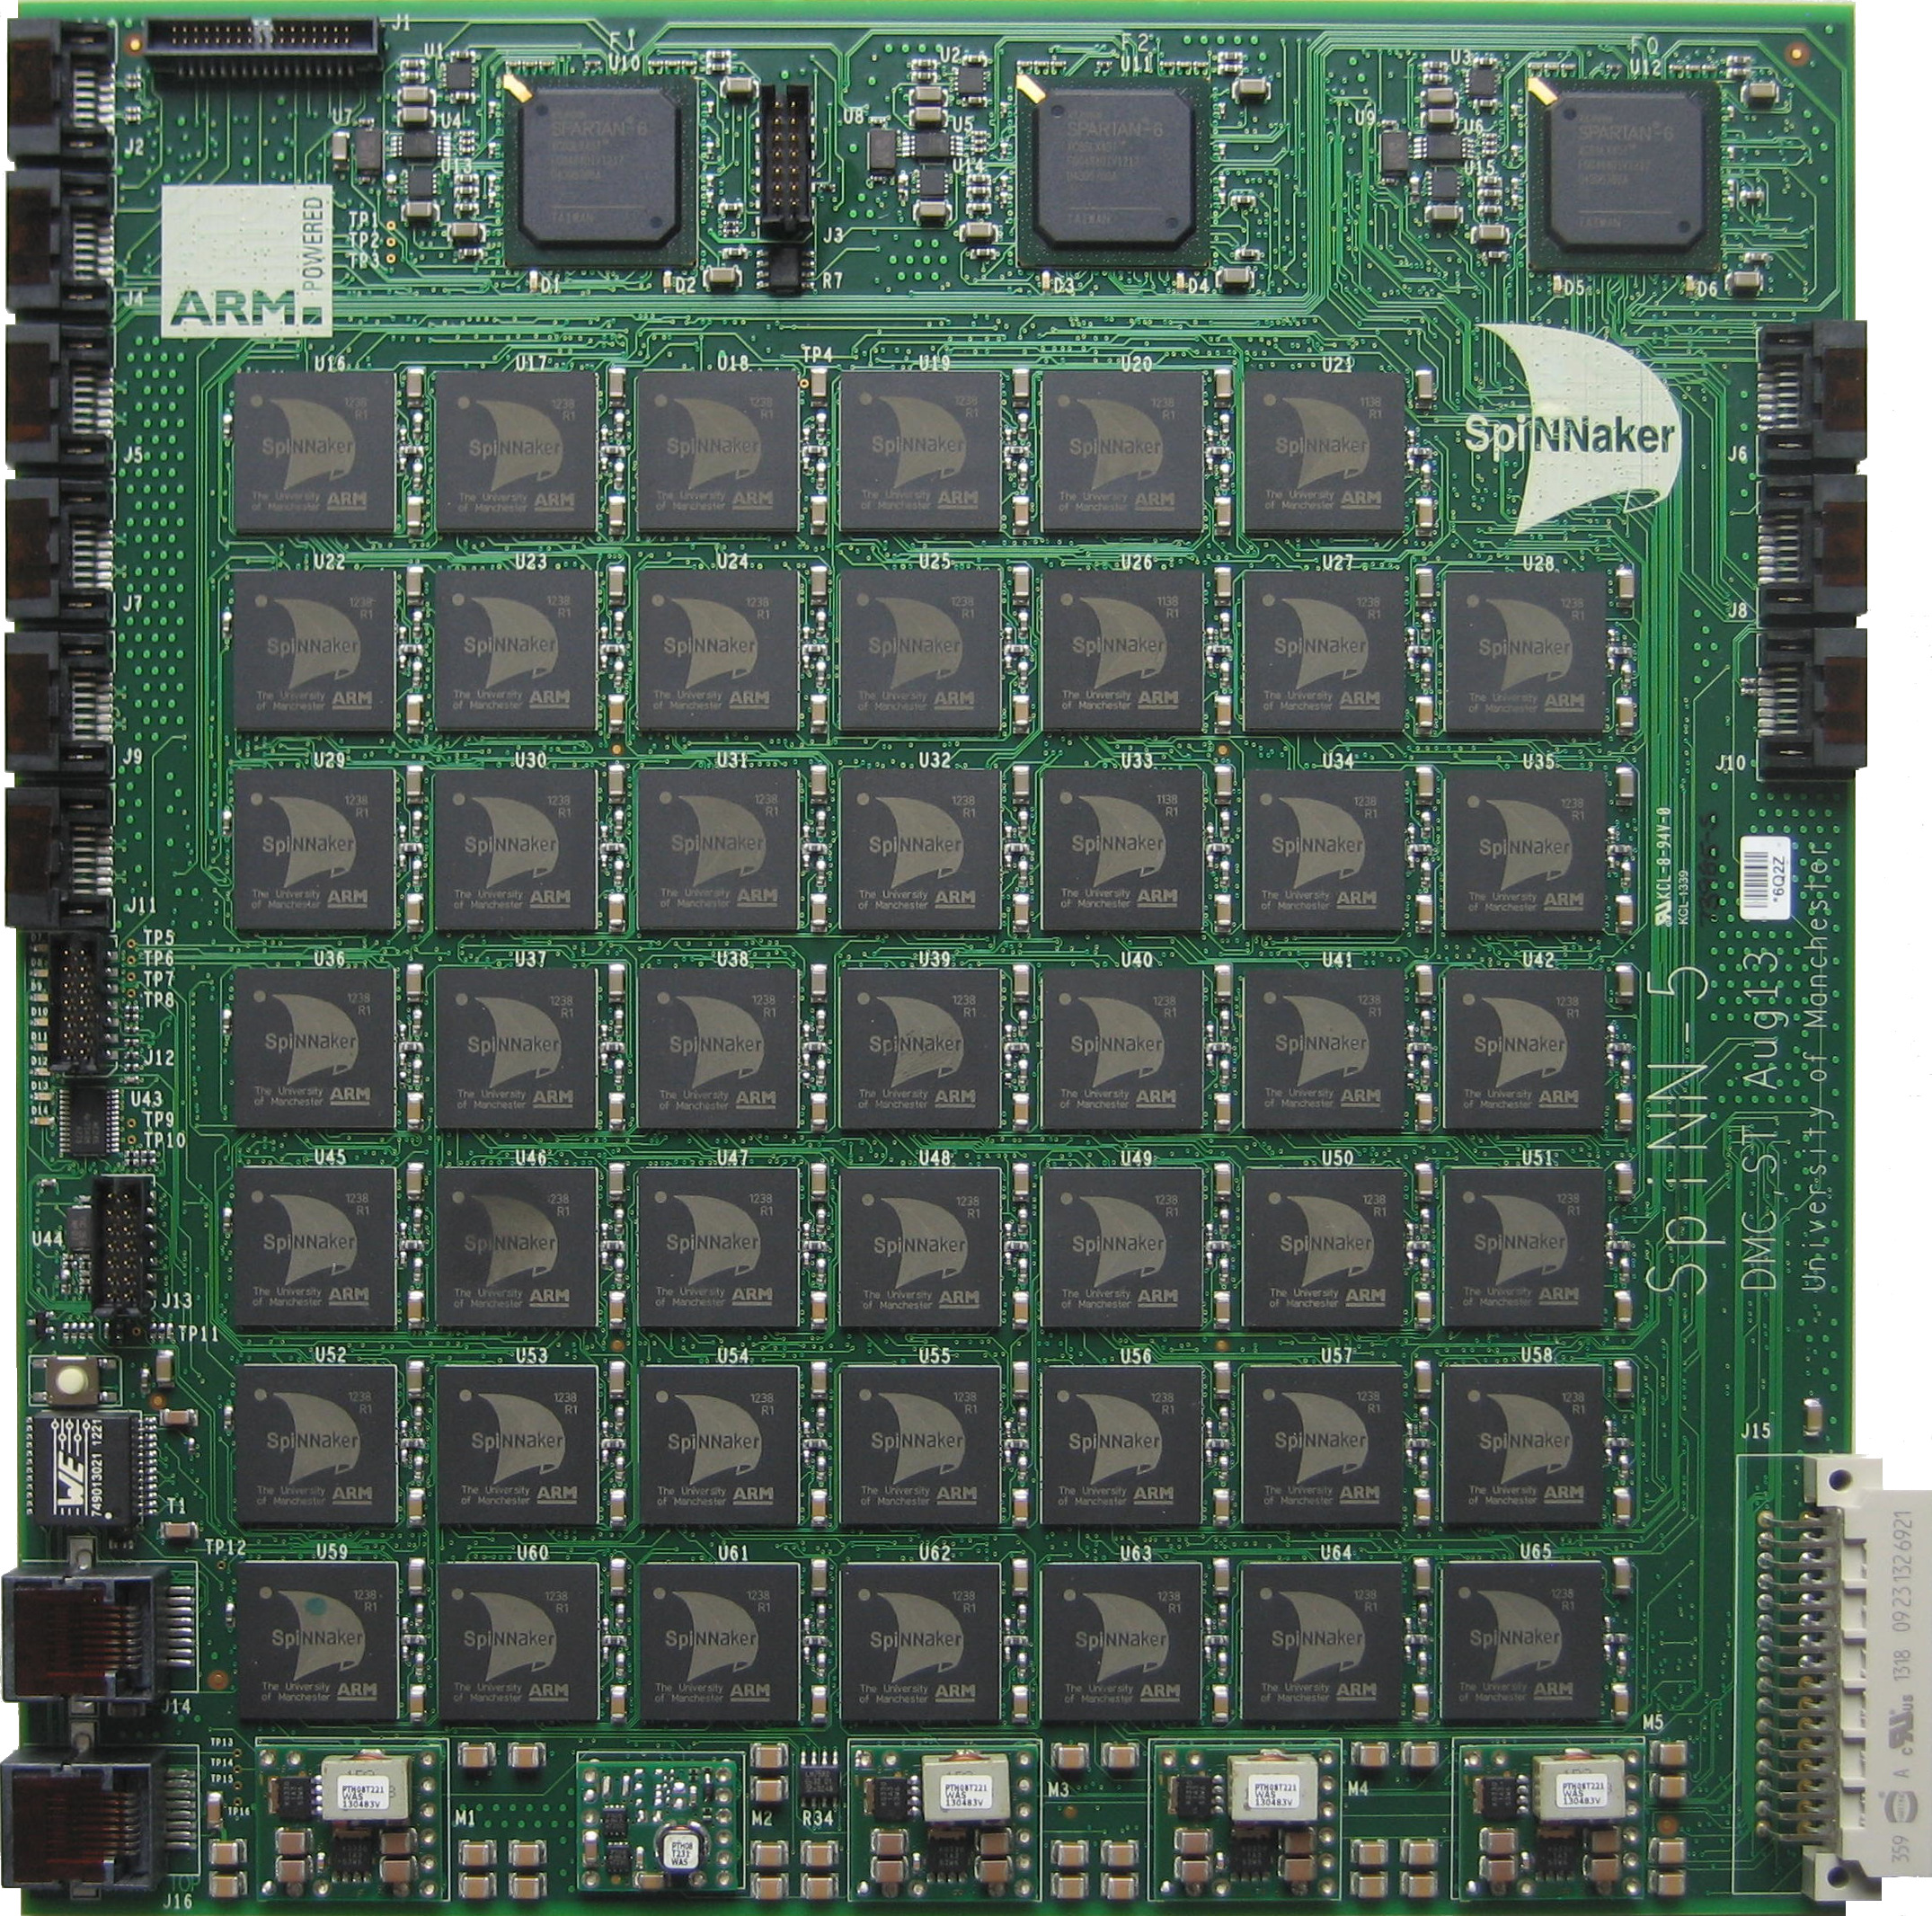
\includegraphics[width=\linewidth]{figures/spinnakerBoard.jpg}
				
				\caption{A SpiNNaker board}
				\label{fig:spinnakerBoard}
			\end{subfigure}
			~~~
			\begin{subfigure}[b]{0.45\linewidth}
				\center
				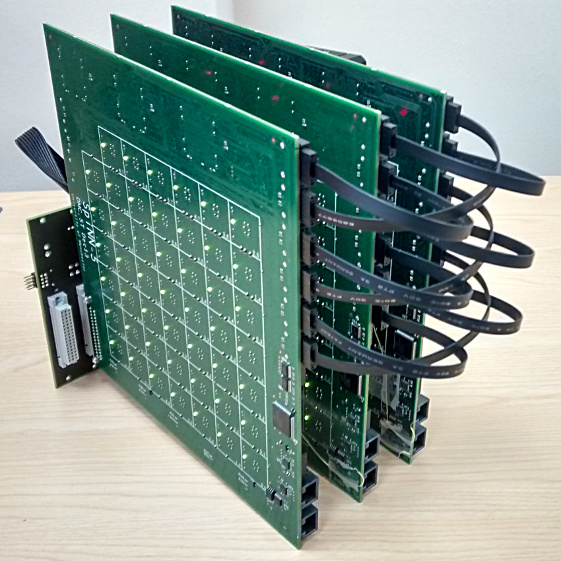
\includegraphics[width=\linewidth]{figures/threeboard.jpg}
				
				\caption{Three board system}
				\label{fig:threeboard}
			\end{subfigure}
			
			\vspace*{2em}
			
			\begin{subfigure}{\linewidth}
				\center
				\buildfig{figures/sata-connections.tex}
				
				\caption{The logical connectivity between chips in multi-board systems.
				Each board's forty-eight chips (drawn here as hexagons) form a wrapped
				triple. Connections between chips on neighbouring boards are
				concentrated onto a single HSS link.}
				\label{fig:sata-connections} \end{subfigure}
			
			\caption{SpiNNaker boards.}
			\label{fig:spinnaker-boards}
		\end{figure}
		
		To build large SpiNNaker systems comprising of tens of thousands of
		SpiNNaker chips, groups of forty-eight chips are mounted onto circuit
		boards as illustrated in figure~\ref{fig:spinnakerBoard}. These boards may
		be connected together to form larger systems.  Figure~\ref{fig:threeboard}
		shows a prototype three board system configured as a $12\times12$ hexagonal
		torus.
		
		Though the chips are physically arranged in a (nearly) $7\times7$ grid on
		each SpiNNaker board, they logically form a `wrapped triple'
		\cite{davidsonWiring}, a shape described in detail in appendix
		\ref{sec:partitioning} and illustrated in
		figure~\ref{fig:sata-connections}. Logically, the chips at the periphery of
		each board connect to their neighbours on adjacent boards. Normally
		SpiNNaker chips connect using a low power, asynchronous 2-of-7 protocol
		requiring sixteen wires per bidirectional chip-to-chip link
		\cite{bainbridge03}. If this link technology were used to connect chips on
		neighbouring boards, each pair of boards would need to be connected with a
		128~wire cable. Cables and connectors supporting this many signals are
		expensive and physically large making them unsuitable for use with
		SpiNNaker. Instead, chip-to-chip connections between boards are multiplexed
		and demultiplexed onto a single High-Speed Serial (HSS) link
		\cite{athavale05} carried via commodity S-ATA cables often used to connect
		hard disks in desktop computers and servers \cite{sata3spec}.  The six
		high-speed links are implemented by three onboard FPGAs (the three large
		chips at the top of the SpiNNaker board) and are logically transparent to
		the underlying network.
		
		In chapter~\ref{sec:building} I describe how very large SpiNNaker machines
		may be constructed using over one thousand SpiNNaker boards.
